\documentclass{article}

\usepackage{graphicx}
\usepackage{amsmath}

\usepackage[margin=1in]{geometry}


\def\hwtitle{Computational Physics HW1}
\def\hwauthor{Ethan Rooney}
\def\hwdate{2020-01-29}

\usepackage{fancyhdr}
\lhead{\hwauthor}
\chead{\hwtitle}
\rhead{\hwdate}
\lfoot{\hwauthor}
\cfoot{}
\rfoot{\thepage}
\renewcommand{\footrulewidth}{0.4pt}
\pagestyle{fancy}

\author{\hwauthor}
\title{\hwtitle}
\date{\hwdate}

\begin{document}

\maketitle
\thispagestyle{fancy}

\section{Introduction}

A harmonic occilator is defined by a system that experiances a restoritive force proportional to its displacement from it's rest location. This is known as Hook's Law and the mathematical form is seen in \( F_{x} \eq \minus kx \). \( F_x \) is the force on the object. \( k \) is an arbitrary constant determined by the physical properties of a system (i.e. for a spring k would be determined by the stiffness of the material).  \( x \) is the displacement of an object from its "rest" position.
  

This Homework deals with a special case where an object follows this law in X and Y independantly.
As such it is governed by the following  \ref{eq:2}. \( A \) is the maximum amplitude reached by the system in a particular direction. \( omega \eq \sqrt{k/m} \). 
\( m \) is the mass of the object occelating. \( phi \) is the inital phase position of the system.

\begin{equation} \label{eq:2}
	x(t)\eq A_x\sin(\omega_xt+\phi_x)
	y(t)\eq A_y\sin(\omega_{y}t+\phi_{y})
\end{equation}

The first part of the homework deals with cases when \( \omega_x \) and \( \omega_y \) are equal. 

For the Bonus Problems I will explore some of the possibilites when \( \omega_x \) and \( \omega_y \)
are varied independently.

\section{Results}

\bigskip
\noindent{\bf Question 1}
\medskip

Code submitted on Blackboard

\bigskip
\noindent{\bf Question 2}
\medskip

See attached \ref{plots}

\bigskip
\noindent{\bf Question 3}
\medskip

If \( \omega_x \eq \omega_y \) then the range of shapes possible are rather limited. The variation is from perfectly circular to a line. As \( \Delta\phi \) grows from \( 0 \) to \( \pi \) the shape transitions from a line, of \( y \eq A_x / A_yx \), through an eliptical shape to a circle, at \( \Delta\phi \eq \pi \), then back to a line, of \( y \eq -A_x / A_y \times x \).


\bigskip
\noindent{\bf Bonus 1}
\medskip

For small ratios of \( \omega_x \) and \( \omega_y \) a closed loop was formed and the pattern would repeat like the center plot in \ref{lissa}, so long as \( \Delta\phi \neq n\pi \) where \( \n \) is an integer. If \( n \) is an integer, then instead of "looping" the system will occilate back and forth along a single path like scene in the first plot in \ref{lissa}.

\bigskip
\noindent{\bf Bonus 2}
\medskip

If the ratios of \( \omega_x \) and \( \omega_{y} \) are irrational numbers i.e. \( \sqrt{5} \) like seen in the right most plot of \ref{lissa}, then the system cannot repeat. This leads to what appears to be random dots. But if you look carefully you can see a structure to the dot. The system can almost, but not quite loop bak over itself and leave a series of nearly parallel paths.

\section{Conclusions}

Main challenges faced in this coding project were discovering the "-lm" flag for gcc. It also served a good refresher on how to work with c.
Furthermore, I had never worked with Mathematica before, discovering some of its' features for the first time was fun.

\section{Plots} \label{plots}
\begin{figure}[b]
\begin{center}
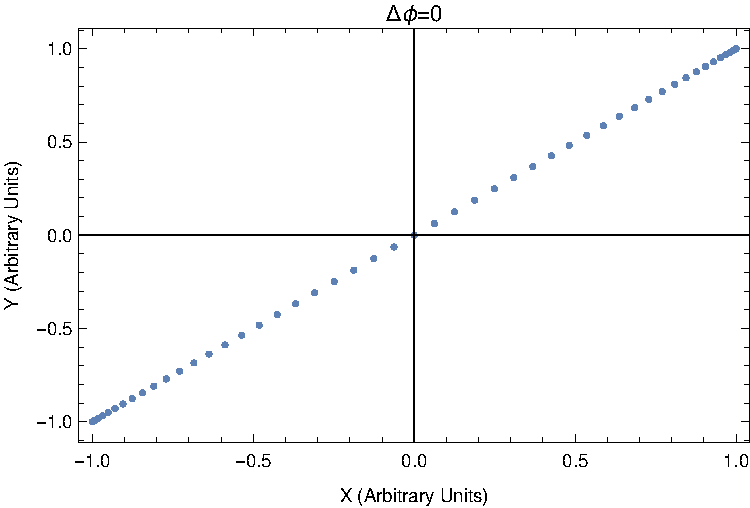
\includegraphics[width=0.25\textwidth]{plot1.pdf}
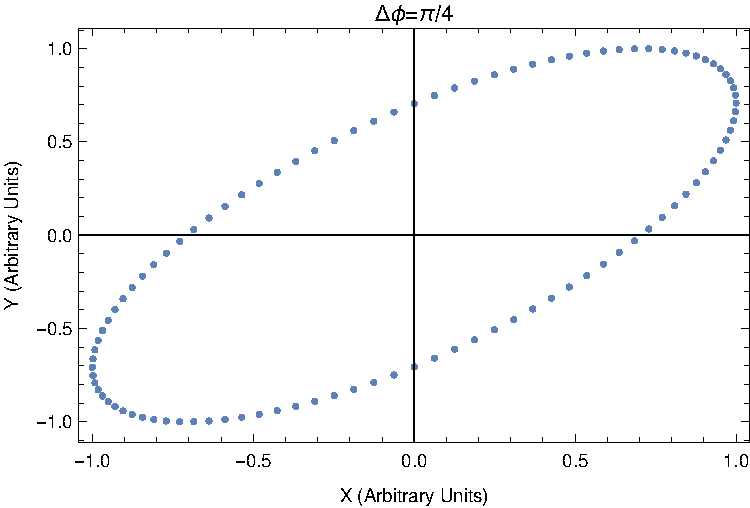
\includegraphics[width=0.25\textwidth]{plot2.pdf}
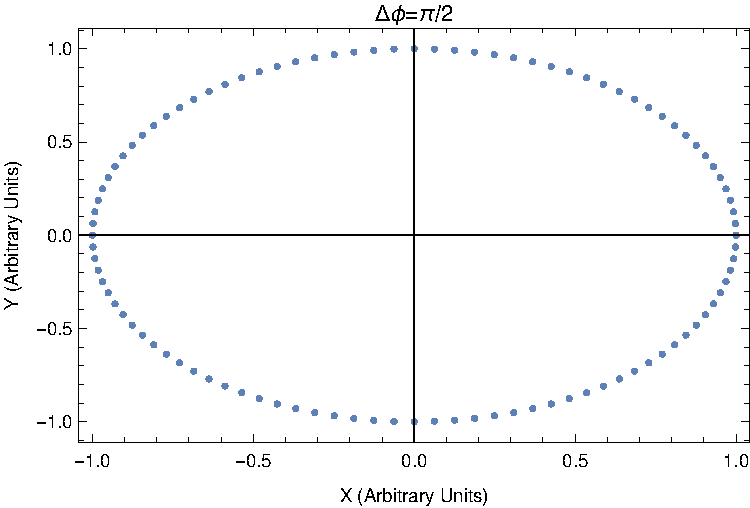
\includegraphics[width=0.25\textwidth]{plot3.pdf}
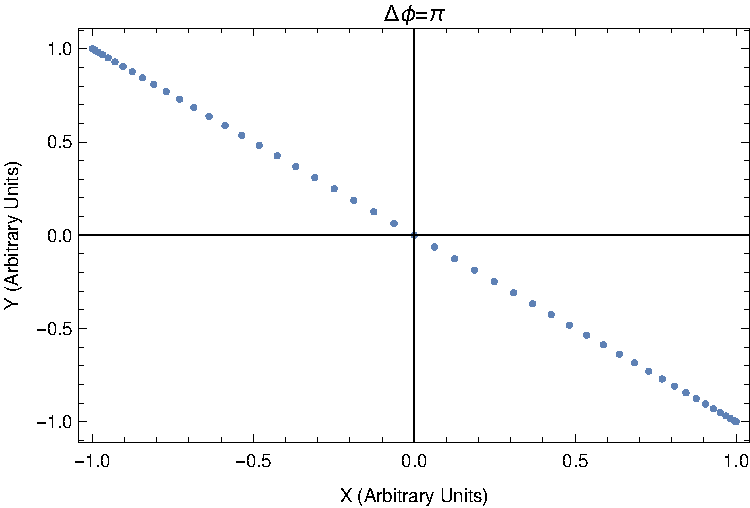
\includegraphics[width=0.25\textwidth]{plot4.pdf}
\end{center}
\caption{These plots above show the types of shapes possible to make using this system of harmonic occilaters.}
\end{figure}

\begin{figure}[b]
\begin{center}
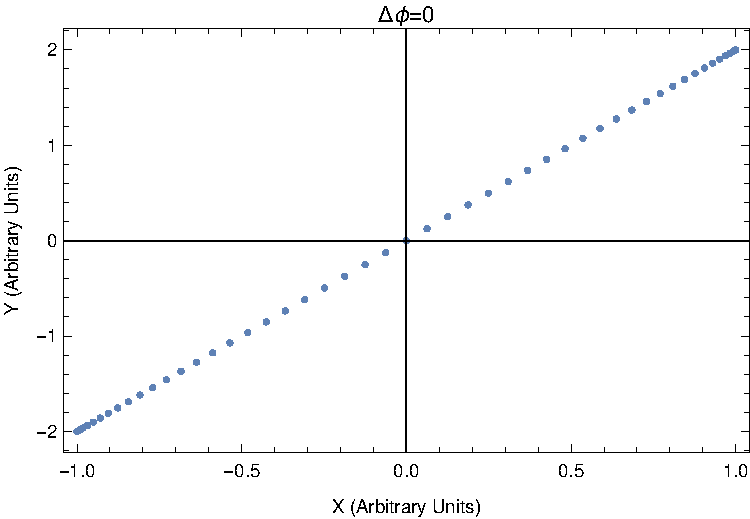
\includegraphics[width=0.25\textwidth]{plot5.pdf}
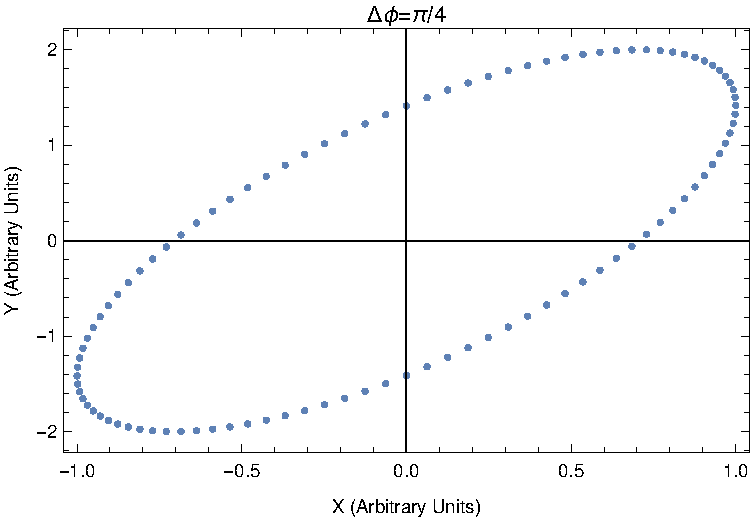
\includegraphics[width=0.25\textwidth]{plot6.pdf}
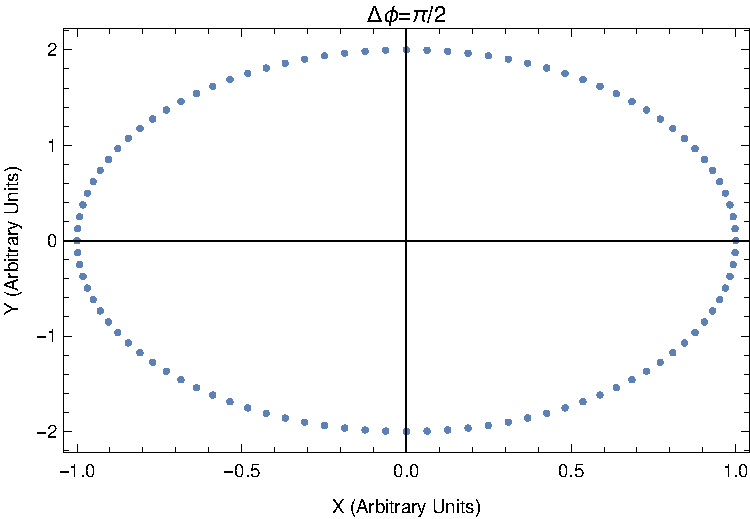
\includegraphics[width=0.25\textwidth]{plot7.pdf}
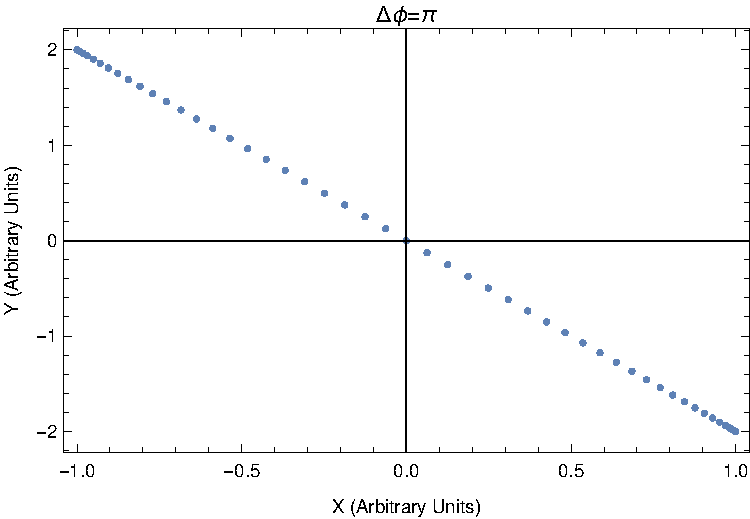
\includegraphics[width=0.25\textwidth]{plot8.pdf}
\end{center}
\caption{These plots are nearly identical to the plots above, with the exception that in the amplitude in the y direction is twice what it would be in the corrisponding picture above.}
\end{figure}

\begin{figure}[b]
\begin{center}
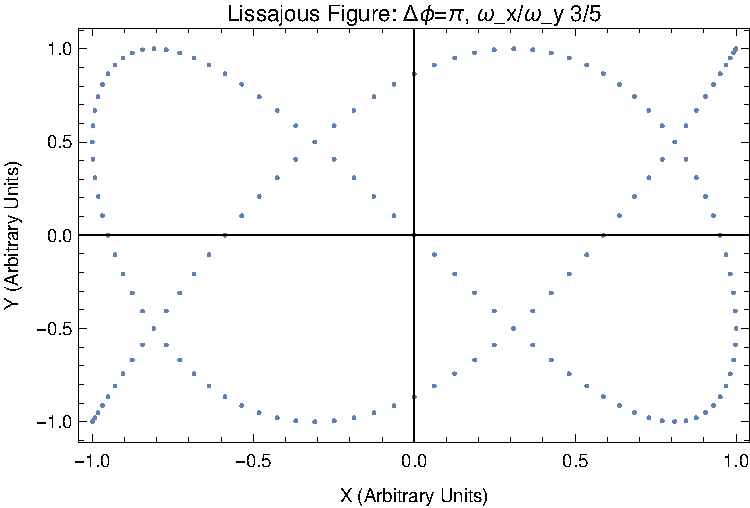
\includegraphics[width=0.33\textwidth]{plot9.pdf}
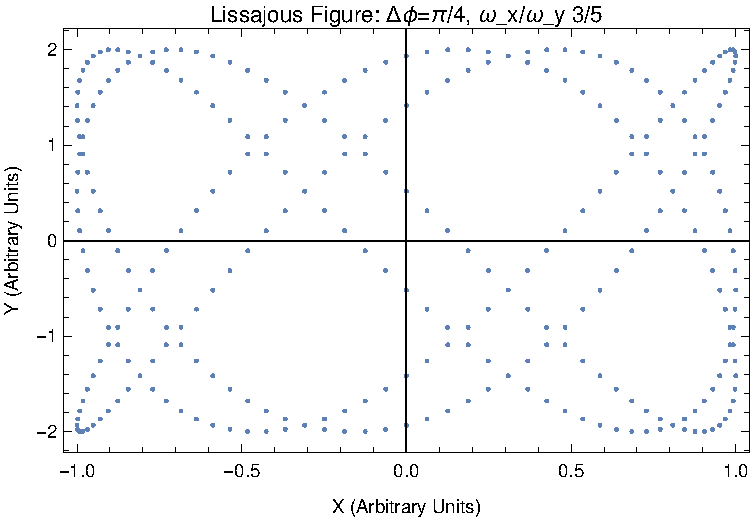
\includegraphics[width=0.33\textwidth]{plot10.pdf}
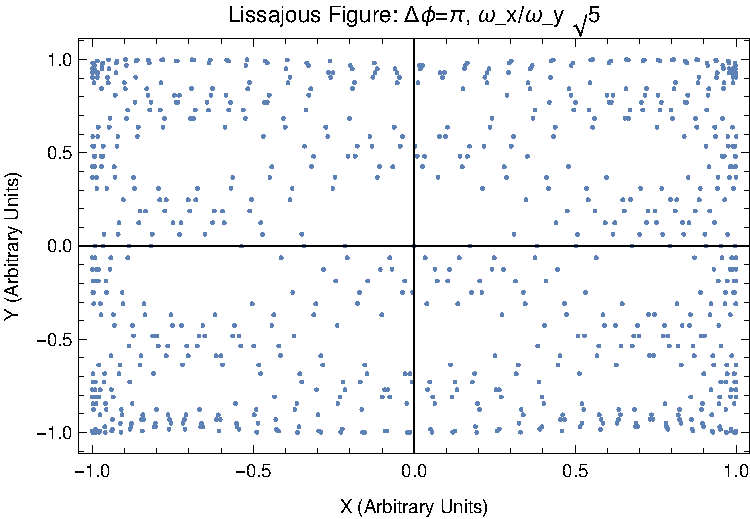
\includegraphics[width=0.33\textwidth]{plot11.pdf}
\end{center}
\caption{Seen above are some of the patterns formed by Lassajous figures}
\label{lissa}
\end{figure}

\end{document}
